Mit der erarbeiteten Variante aus dem System Engineering wurde zunächst ein Blockschaltbild erstellt. Dieses ist in Abbildung \ref{pics:blockschaltbild} dargestellt. In diesem wurden bereits einige Komponenten ausgewählt: 
\paragraph{MILAN Modul MT32-TDM to MILAN} Die Firma \href{https://www.joyned.at/}{JOYNED GmbH} bietet auf ihrem Webshop bereits ein fix-fertiges Milan-Modul an, welches über PoE gespiesen wird und 16x16 Audiokanäle verarbeiten kann (siehe \cite{joyned_store}). Abbildung \ref{pics:mt32_TDM} zeigt das Modul. Zum Anschluss in einem Gerät dient ein System Connector, welches nebst den Datensignalen in TDM-Format (\textbf{Time Division Multiplex}) auch Master Clock-, I$^{2}$C-, GPIO-, 3V- und 5V-Leitungen besitzt.
\begin{figure}[H]
	\centering
	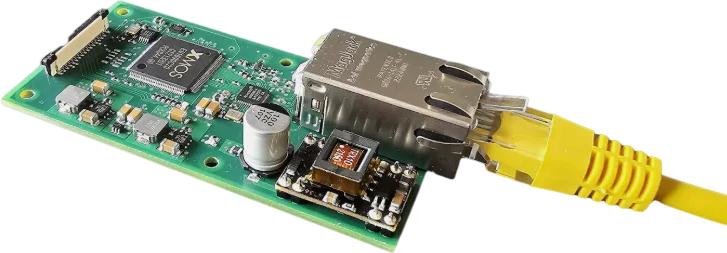
\includegraphics[width=\textwidth*3/4]{pictures/Joyned_MT32-TDM.png}
	\caption{Das Milan-Modul der Firma Joyned GmbH}
	\label{pics:mt32_TDM}
\end{figure}
\paragraph{Gehäuse}Das Gehäuse wurde schon in der Vorarbeit gezeichnet und war daher schon gegeben. Auf einem länglicher Resonanzkasten sind sechs Membran-Platten angebracht, die unabhängig voneinander in Schwingung gebracht werden können. Zusätzlich ist auch eine Aussparung für die Elektronik vorgesehen. Abbildung \ref{pics:render_box} zeigt eine grafische Darstellung davon.
\begin{figure}[H]
	\centering
	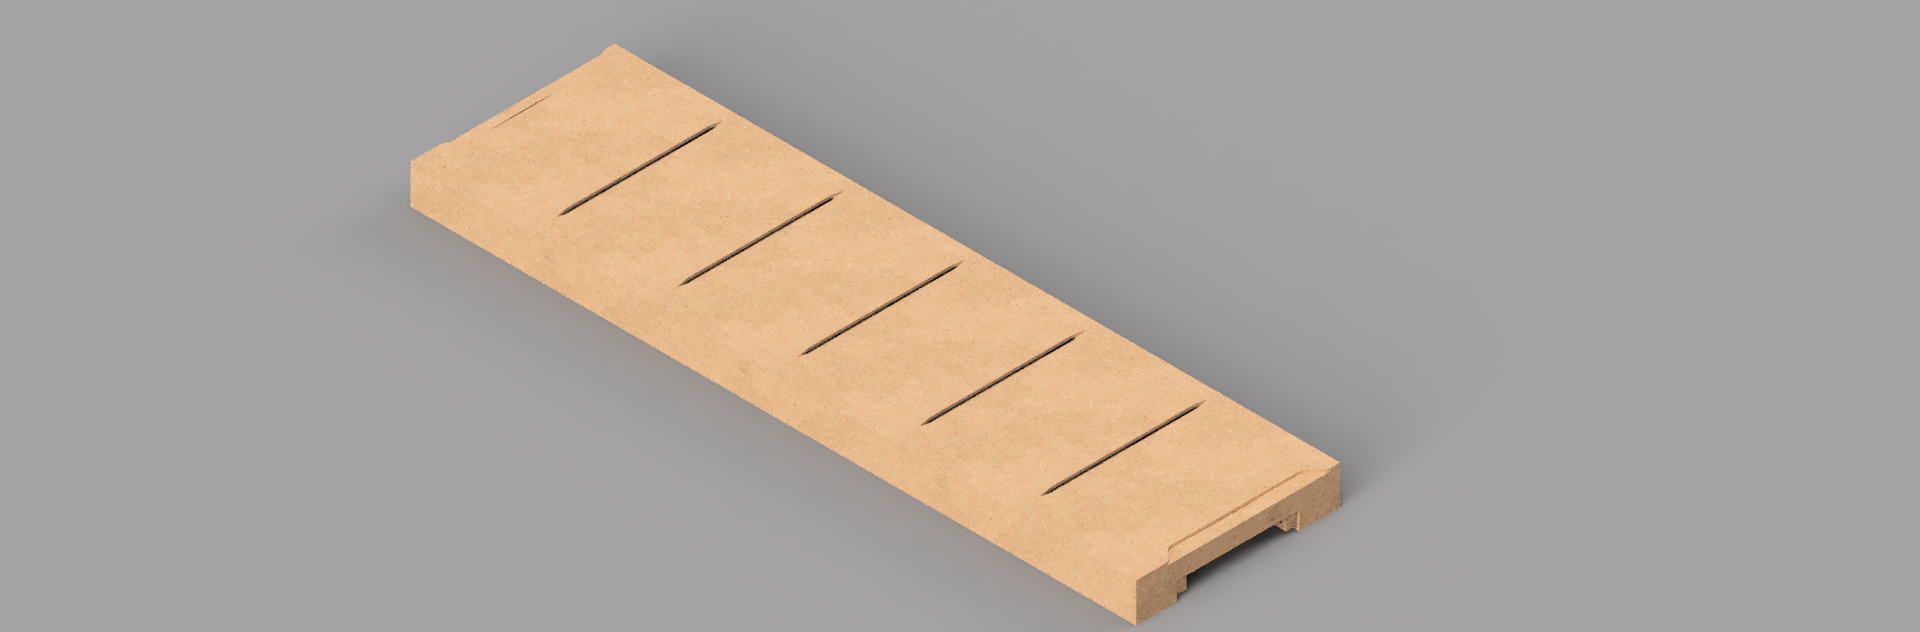
\includegraphics[width=\textwidth]{pictures/Nathophone_2025-Sep-29_07-57-22AM-000_CustomizedView2892546826.png}
	\caption{Das Gehäuse mit 6 Frontplatten}
	\label{pics:render_box}
\end{figure}
\begin{figure}[H]
	\centering
	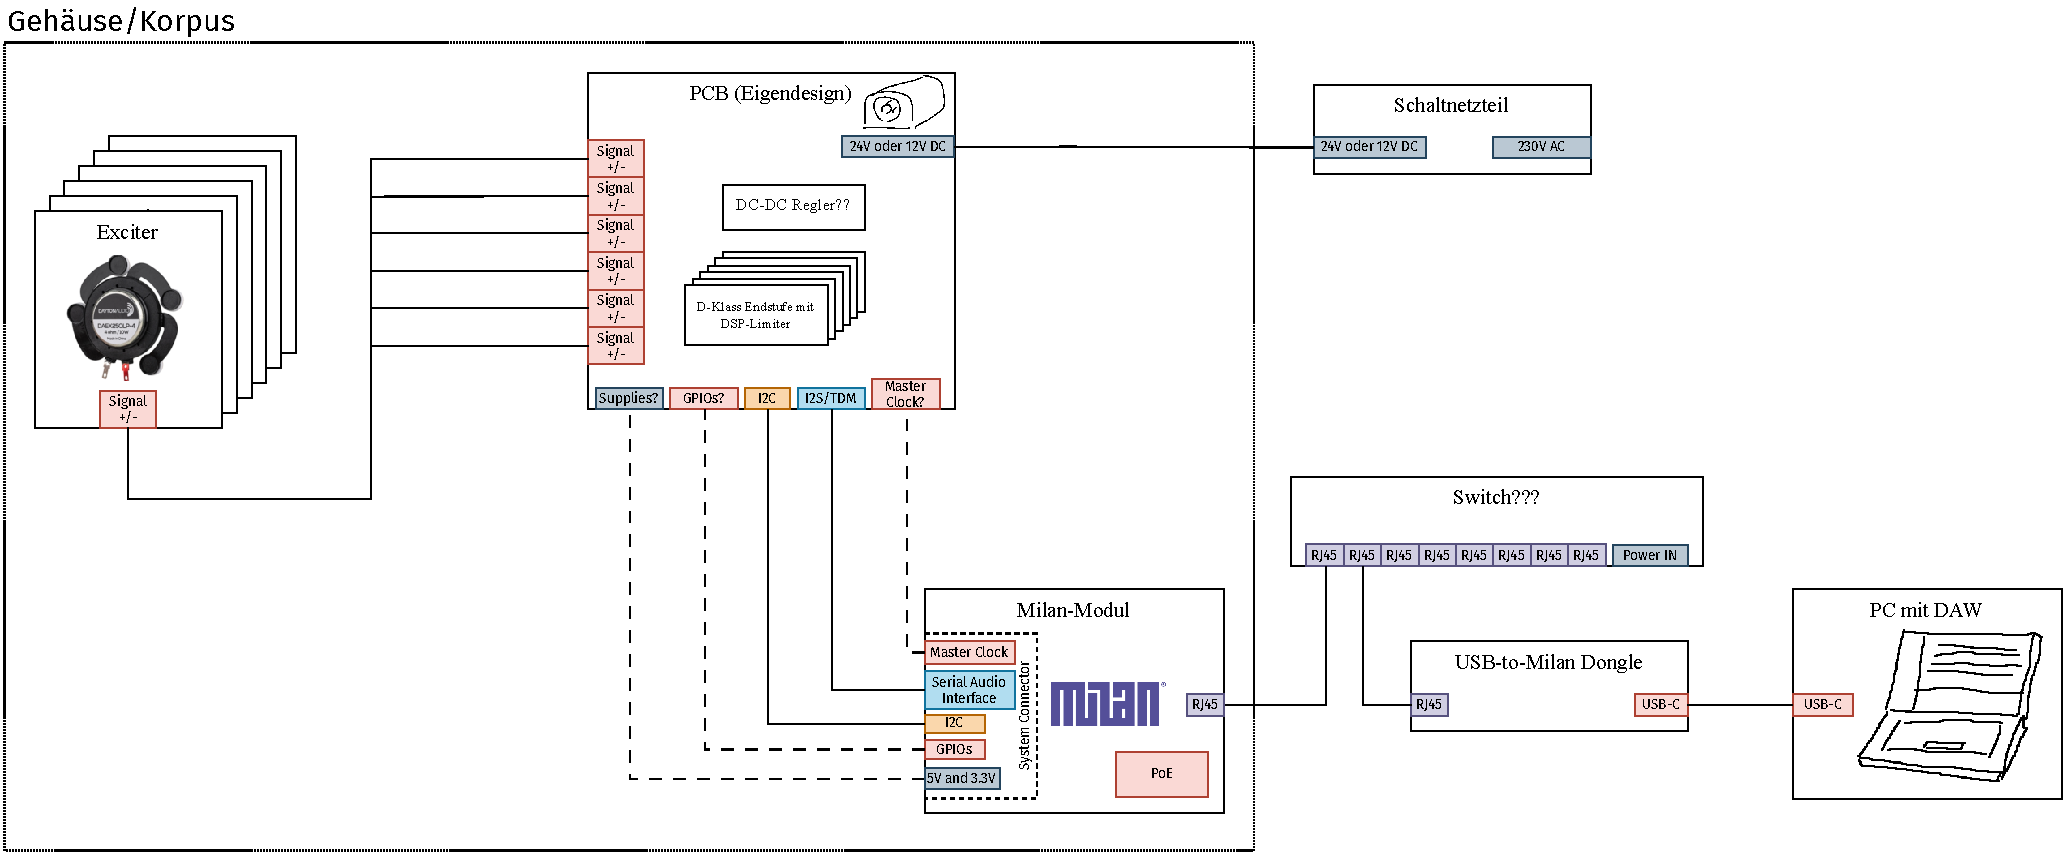
\includegraphics[width=\textwidth]{pictures/blockschaltbild.pdf}
	\caption{Das Blockschaltbild}
	\label{pics:blockschaltbild}
\end{figure}
Bei der Erstellung wurde schnell klar, dass auch noch einige undefinierte Komponenten vorhanden waren. So muss unter Umständen die interne Spannungsregelung noch definiert werden, da die externe Speisung direkt als Endstufenspeisung zu verwenden in der Regel keine gute Idee ist, da z.B. so eine Überwachung und Regelung der Stromaufnahme nur passiv und mit einem Leistungsverlust realisiert werden kann.
\\Zudem war noch unklar, ob der USB-Milan Dongle direkt auf das Modul verbunden werden kann (evtl. über einen PoE-Injector\footnote{Ein Gerät, welches einer Ethernet-Verbindung eine PoE-Speisespannung hinzufügt und seriell in die Verbindung geschaltet wird.}) oder über einen Milan-fähigen Switch verbunden werden muss.
\\Des weiteren war noch nicht klar, ob nebst den Datenleitungen des Moduls (Serial Audio Interface und I2C) auch noch die anderen Signale wie Master Clock etc. verwendet werden müssen.
\\Als letzter Punkt musste noch abgeklärt werden, ob das Modul zwingend mit PoE, oder ob auch über den System Connector gespiesen werden kann. Also 3V- und 5V-Pins als Eingänge.